% TEMPLATE for Usenix papers, specifically to meet requirements of
%  USENIX '05
% originally a template for producing IEEE-format articles using LaTeX.
%   written by Matthew Ward, CS Department, Worcester Polytechnic Institute.
% adapted by David Beazley for his excellent SWIG paper in Proceedings,
%   Tcl 96
% turned into a smartass generic template by De Clarke, with thanks to
%   both the above pioneers
% use at your own risk.  Complaints to /dev/null.
% make it two column with no page numbering, default is 10 point

% Munged by Fred Douglis <douglis@research.att.com> 10/97 to separate
% the .sty file from the LaTeX source template, so that people can
% more easily include the .sty file into an existing document.  Also
% changed to more closely follow the style guidelines as represented
% by the Word sample file. 

% Note that since 2010, USENIX does not require endnotes. If you want
% foot of page notes, don't include the endnotes package in the 
% usepackage command, below.

% This version uses the latex2e styles, not the very ancient 2.09 stuff.

% Updated July 2018: Text block size changed from 6.5" to 7"

\documentclass[letterpaper,twocolumn,10pt]{article}
\usepackage{int,graphicx,endnotes}
\begin{document}

%don't want date printed
\date{}

%make title bold and 14 pt font (Latex default is non-bold, 16 pt)
\title{\Large \bf Wonderful : A Terrific Application and Fascinating Paper}

%for single author (just remove % characters)
\author{
{\rm Your N.\ Here}\\
Your Institution
\and
{\rm Second Name}\\
Second Institution
% copy the following lines to add more authors
% \and
% {\rm Name}\\
%Name Institution
} % end author

\maketitle

\subsection*{Abstract}
Your Abstract Text Goes Here.  Just a few facts.
Whet our appetites.

\section{Introduction}

A paragraph of text goes here.  Lots of text.  Plenty of interesting
text. \\

More fascinating text. Features\endnote{Remember to use endnotes, not footnotes!} galore, plethora of promises.\\

\section{This is Another Section}

Some embedded literal typset code might 
look like the following :

{\tt \small
\begin{verbatim}
int wrap_fact(ClientData clientData,
              Tcl_Interp *interp,
              int argc, char *argv[]) {
    int result;
    int arg0;
    if (argc != 2) {
        interp->result = "wrong # args";
        return TCL_ERROR;
    }
    arg0 = atoi(argv[1]);
    result = fact(arg0);
    sprintf(interp->result,"%d",result);
    return TCL_OK;
}
\end{verbatim}
}

Now we're going to cite somebody.  Watch for the cite tag.
Here it comes~\cite{Chaum1981,Diffie1976}.  The tilde character (\~{})
in the source means a non-breaking space.  This way, your reference will
always be attached to the word that preceded it, instead of going to the
next line.

\section{This Section has SubSections}
\subsection{First SubSection}

Here's a typical figure reference.  The figure is centered at the
top of the column.  It's scaled.  It's explicitly placed.  You'll
have to tweak the numbers to get what you want.\\

\begin{figure}[h]
\begin{center}
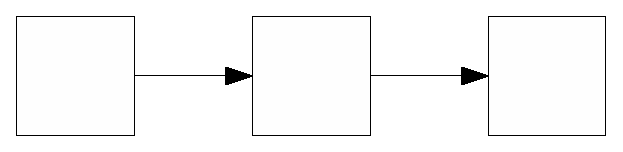
\includegraphics[width=0.5\textwidth]{figures/fig1.eps}
\end{center}
\caption{Wonderful Flowchart}
\end{figure}

This text came after the figure, so we'll casually refer to Figure 1
as we go on our merry way.

\subsection{New Subsection}

It can get tricky typesetting Tcl and C code in LaTeX because they share
a lot of mystical feelings about certain magic characters.  You
will have to do a lot of escaping to typeset curly braces and percent
signs, for example, like this:
``The {\tt \%module} directive
sets the name of the initialization function.  This is optional, but is
recommended if building a Tcl 7.5 module.
Everything inside the {\tt \%\{, \%\}}
block is copied directly into the output. allowing the inclusion of
header files and additional C code." \\

Sometimes you want to really call attention to a piece of text.  You
can center it in the column like this:
\begin{center}
{\tt \_1008e614\_Vector\_p}
\end{center}
and people will really notice it.\\

\noindent
The noindent at the start of this paragraph makes it clear that it's
a continuation of the preceding text, not a new para in its own right.


Now this is an ingenious way to get a forced space.
{\tt Real~$*$} and {\tt double~$*$} are equivalent. 

Now here is another way to call attention to a line of code, but instead
of centering it, we noindent and bold it.\\

\noindent
{\bf \tt size\_t : fread ptr size nobj stream } \\

And here we have made an indented para like a definition tag (dt)
in HTML.  You don't need a surrounding list macro pair.
\begin{itemize}
\item[]  {\tt fread} reads from {\tt stream} into the array {\tt ptr} at
most {\tt nobj} objects of size {\tt size}.   {\tt fread} returns
the number of objects read. 
\end{itemize}
This concludes the definitions tag.

\subsection{How to Build Your Paper}

You have to run {\tt latex} once to prepare your references for
munging.  Then run {\tt bibtex} to build your bibliography metadata.
Then run {\tt latex} twice to ensure all references have been resolved.
If your source file is called {\tt intTemplate.tex} and your {\tt
  bibtex} file is called {\tt intTemplate.bib}, here's what you do:
{\tt \small
\begin{verbatim}
latex intTemplate
bibtex intTemplate
latex intTemplate
latex intTemplate
\end{verbatim}
}


\subsection{Last SubSection}

Well, it's getting boring isn't it.  This is the last subsection
before we wrap it up.

\section{Acknowledgments}

A polite author always includes acknowledgments.  Thank everyone,
especially those who funded the work. 

\section{Availability}

It's great when this section says that MyWonderfulApp is free software, 
available via anonymous FTP from

\begin{center}
{\tt ftp.site.dom/pub/myname/Wonderful}\\
\end{center}

Also, it's even greater when you can write that information is also 
available on the Wonderful homepage at 

\begin{center}
{\tt http://www.site.dom/\~{}myname/SWIG}
\end{center}

Now we get serious and fill in those references.  Remember you will
have to run latex twice on the document in order to resolve those
cite tags you met earlier.  This is where they get resolved.
We've preserved some real ones in addition to the template-speak.
After the bibliography you are DONE.

{\normalsize \bibliographystyle{acm}
\bibliography{int}}


\theendnotes

\end{document}
